\clearpage
\section{Final Dataset}
Upon analysing the available datasets, it was 
decided to use several of them for specific purposes. 


%%%
\subsection{Pan et al tested dataset}
\label{section:Pan et al tested dataset}
The analysis of the dataset by Pan et al.\ 
enabled the construction of a small dataset 
consisting of definitively correct and definitively 
incorrect code samples (where “incorrect” refers to 
cases in which the LLM-generated code did not produce 
the same outputs as the corresponding human-written code).

The process began with the subset of the dataset 
corresponding to the prompt \textit{“Removal of 
stop words from the prompt”}, which includes 5069 
samples. From this subset, has been discarded all code 
samples that the framework was unable to process. 
Tests were then executed on the remaining samples, 
and only those which did not produce runtime faults 
were retained—this was necessary to exclude failures 
due to incorrectly generated tests or missing import 
statements.

As a result, a dataset of approximately 1000 code 
samples was obtained, of which around 600 were 
classified as correct and 400 as incorrect (i.e., 
they failed at least one test).



\begin{figure}[H]
    \centering
    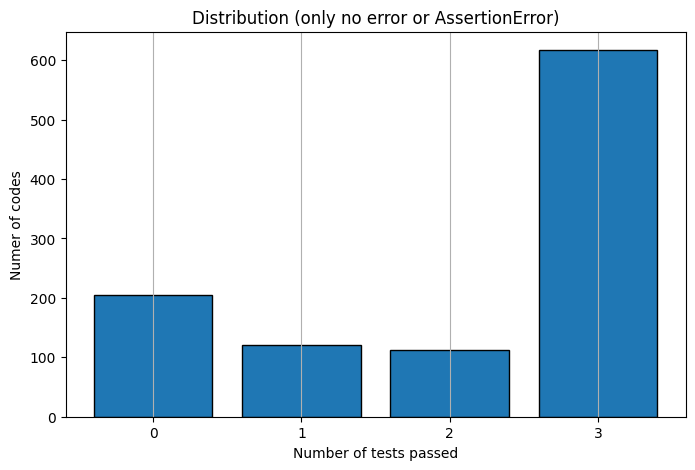
\includegraphics[width=0.4\textwidth]{img/panetaltest/600600.png}
    \caption{Source distribution}
    \label{fig:panetaltest_600600}
\end{figure}


%%%
\subsection{Dataset standardization}

Different \textit{"roles"} have therefore been assigned to the datasets in the 
testing process.


CodeMirage \ref{section:CoDet-M4}  is the primary test dataset, against which all methods will be compared. 
This choice is motivated by the fact that CodeMirage has already published 
tests on various methods using its dataset, providing a solid starting point. 
Additionally, the CodeMirage dataset is the most diverse and extensive: 
it contains both short code snippets and entire programs, includes 10 
programming languages, and 10 different LLMs. This dataset is therefore 
useful for evaluating the generalization of results across multiple 
programming languages and LLMs.


AIGCodeSet \ref{section:AiGCodeSet} plays the role of evaluating, 
among a set of methods selected 
through the tests on CodeMirage, the effectiveness on competitive-type code. 
Competitive code is an extremely important type of code because it requires the 
greatest detection capabilities. This is because competitive code refers to 
coding exercises, such as those requested during job interviews and in educational 
settings. Additionally, AIGCodeSet can also be used to make secondary considerations 
about the detection method's capabilities on more complex code.


The code from Pan et al. tested \ref{section:Pan et al tested dataset} using the framework developed in 
\ref{section:Test framework} allows us to assess the considerations 
of various works regarding the increased difficulty of detecting error-free code. 
This test remains a consideration, and if proven true, it should encourage future 
works to make more intensive use of testing frameworks to improve the quality of 
their datasets, both for training and testing.


CoDet-M4 \ref{section:CoDet-M4} does not appear to be a high-quality dataset, but it remains a 
dataset of enormous size. Therefore, although it is not recommended for testing, 
it could be interesting to use this dataset to train an AI-based detection method 
and evaluate its results.

So the final role of the dataset will be:

\begin{itemize}
    \item \textbf{CodeMirage:}
    \begin{itemize}
        \item Language generalization
        \item LLMs Generalization
    \end{itemize}

    \item \textbf{AIGCodeSet:}
    \begin{itemize}
        \item competitive code evaluation
        \item difference between difficulty
    \end{itemize}

    \item \textbf{Pan:}
    \begin{itemize}
        \item correct code vs wrong code evaluation
    \end{itemize}

    \item \textbf{CoDET-M4:}
    \begin{itemize}
        \item Traning set for AI based detection
    \end{itemize}
\end{itemize}



